\documentclass[lecture.tex]{subfiles}

\begin{document}

\exercice{Wissam Benmalek}
%\video{https://youtu.be/blablabla}
\enonce{rdm-0020}{Réaction d'un pont sous chargement}

\begin{figure}[h]
  \centering
  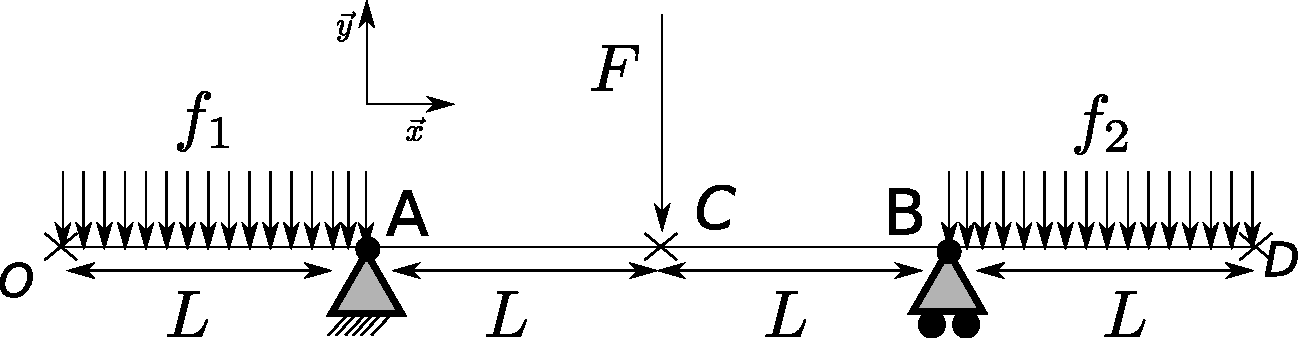
\includegraphics[scale=0.6]{Poutre_Biappuie_V2.pdf}
  \caption{Modélisation simplifiée du pont}
  \label{Poutre_BiApp}
\end{figure}

Dans ce problème on s'intéresse à la résistance d'un pont suite à un chargement créé par deux locomotives de TGV en arrêt. Dans un premier temps, le pont est modélisé par une poutre en liaison pivot en $A$ et en pivot glissant en $B$ (fig \ref{Poutre_BiApp}). Le chargement du TGV de gauche est modélisé par une force linéique répartie $f_1$ alors que celui de droite par une force linéique répartie $f_2$. Une force centrale ponctuelle est appliquée au centre de la poutre notée $F$. La poutre mesure $4L$ en longueur au total.

\begin{enumerate}
  \item Étudier l'hyperstaticité du système
  \item Identifier les inconnues de liaison.
  \item Combien de coupe faut-il pour étudier les efforts internes du système.
  \item Trouver les efforts internes pour chaque coupe. (\textbf{Attention:} Pour alléger les calculs, exprimez les résultats en fonction des inconnues de liaison et les autres paramètres du problème. \textbf{Ne développez pas l'expression des inconnues de liaison}).
  \item On fournit les données suivantes : $f_1=32000 N/m$, $f_2=1.25\cdot f_1$, $L=25m$ et $F=30KN$. Tracer les graphes des efforts internes.
  \item Enfin, on suppose que les efforts répartis $f_1$ et $f_2$ sont remplacés par leurs résultantes ponctuelles respectivement au centre de la portion $OA$ et au centre de la portion $BD$ de la poutre. Expliquez l'impact de cette nouvelle modélisation sur les efforts internes.
\end{enumerate}

\finenonce{rdm-0020}
\finexercice

\end{document}
